\documentclass[1p]{elsarticle_modified}
%\bibliographystyle{elsarticle-num}

%\usepackage[colorlinks]{hyperref}
%\usepackage{abbrmath_seonhwa} %\Abb, \Ascr, \Acal ,\Abf, \Afrak
\usepackage{amsfonts}
\usepackage{amssymb}
\usepackage{amsmath}
\usepackage{amsthm}
\usepackage{scalefnt}
\usepackage{amsbsy}
\usepackage{kotex}
\usepackage{caption}
\usepackage{subfig}
\usepackage{color}
\usepackage{graphicx}
\usepackage{xcolor} %% white, black, red, green, blue, cyan, magenta, yellow
\usepackage{float}
\usepackage{setspace}
\usepackage{hyperref}

\usepackage{tikz}
\usetikzlibrary{arrows}

\usepackage{multirow}
\usepackage{array} % fixed length table
\usepackage{hhline}

%%%%%%%%%%%%%%%%%%%%%
\makeatletter
\renewcommand*\env@matrix[1][\arraystretch]{%
	\edef\arraystretch{#1}%
	\hskip -\arraycolsep
	\let\@ifnextchar\new@ifnextchar
	\array{*\c@MaxMatrixCols c}}
\makeatother %https://tex.stackexchange.com/questions/14071/how-can-i-increase-the-line-spacing-in-a-matrix
%%%%%%%%%%%%%%%

\usepackage[normalem]{ulem}

\newcommand{\msout}[1]{\ifmmode\text{\sout{\ensuremath{#1}}}\else\sout{#1}\fi}
%SOURCE: \msout is \stkout macro in https://tex.stackexchange.com/questions/20609/strikeout-in-math-mode

\newcommand{\cancel}[1]{
	\ifmmode
	{\color{red}\msout{#1}}
	\else
	{\color{red}\sout{#1}}
	\fi
}

\newcommand{\add}[1]{
	{\color{blue}\uwave{#1}}
}

\newcommand{\replace}[2]{
	\ifmmode
	{\color{red}\msout{#1}}{\color{blue}\uwave{#2}}
	\else
	{\color{red}\sout{#1}}{\color{blue}\uwave{#2}}
	\fi
}

\newcommand{\Sol}{\mathcal{S}} %segment
\newcommand{\D}{D} %diagram
\newcommand{\A}{\mathcal{A}} %arc


%%%%%%%%%%%%%%%%%%%%%%%%%%%%%5 test

\def\sl{\operatorname{\textup{SL}}(2,\Cbb)}
\def\psl{\operatorname{\textup{PSL}}(2,\Cbb)}
\def\quan{\mkern 1mu \triangleright \mkern 1mu}

\theoremstyle{definition}
\newtheorem{thm}{Theorem}[section]
\newtheorem{prop}[thm]{Proposition}
\newtheorem{lem}[thm]{Lemma}
\newtheorem{ques}[thm]{Question}
\newtheorem{cor}[thm]{Corollary}
\newtheorem{defn}[thm]{Definition}
\newtheorem{exam}[thm]{Example}
\newtheorem{rmk}[thm]{Remark}
\newtheorem{alg}[thm]{Algorithm}

\newcommand{\I}{\sqrt{-1}}
\begin{document}

%\begin{frontmatter}
%
%\title{Boundary parabolic representations of knots up to 8 crossings}
%
%%% Group authors per affiliation:
%\author{Yunhi Cho} 
%\address{Department of Mathematics, University of Seoul, Seoul, Korea}
%\ead{yhcho@uos.ac.kr}
%
%
%\author{Seonhwa Kim} %\fnref{s_kim}}
%\address{Center for Geometry and Physics, Institute for Basic Science, Pohang, 37673, Korea}
%\ead{ryeona17@ibs.re.kr}
%
%\author{Hyuk Kim}
%\address{Department of Mathematical Sciences, Seoul National University, Seoul 08826, Korea}
%\ead{hyukkim@snu.ac.kr}
%
%\author{Seokbeom Yoon}
%\address{Department of Mathematical Sciences, Seoul National University, Seoul, 08826,  Korea}
%\ead{sbyoon15@snu.ac.kr}
%
%\begin{abstract}
%We find all boundary parabolic representation of knots up to 8 crossings.
%
%\end{abstract}
%\begin{keyword}
%    \MSC[2010] 57M25 
%\end{keyword}
%
%\end{frontmatter}

%\linenumbers
%\tableofcontents
%
\newcommand\colored[1]{\textcolor{white}{\rule[-0.35ex]{0.8em}{1.4ex}}\kern-0.8em\color{red} #1}%
%\newcommand\colored[1]{\textcolor{white}{ #1}\kern-2.17ex	\textcolor{white}{ #1}\kern-1.81ex	\textcolor{white}{ #1}\kern-2.15ex\color{red}#1	}

{\Large $\underline{12n_{0342}~(K12n_{0342})}$}

\setlength{\tabcolsep}{10pt}
\renewcommand{\arraystretch}{1.6}
\vspace{1cm}\begin{tabular}{m{100pt}>{\centering\arraybackslash}m{274pt}}
\multirow{5}{120pt}{
	\centering
	\includegraphics[width=112pt]{../../../GIT/diagram.site/Diagrams/png/2431_12n_0342.png}\\
\ \ \ A knot diagram\footnotemark}&
\allowdisplaybreaks
\textbf{Linearized knot diagam} \\
\cline{2-2}
 &
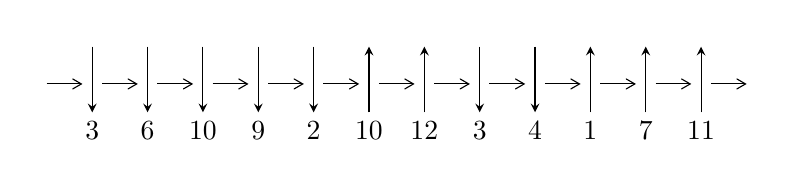
\begin{tikzpicture}[x=20pt, y=17pt]
	% nodes
	\node (C0) at (0, 0) {};
	\node (C1) at (1, 0) {};
	\node (C1U) at (1, +1) {};
	\node (C1D) at (1, -1) {3};

	\node (C2) at (2, 0) {};
	\node (C2U) at (2, +1) {};
	\node (C2D) at (2, -1) {6};

	\node (C3) at (3, 0) {};
	\node (C3U) at (3, +1) {};
	\node (C3D) at (3, -1) {10};

	\node (C4) at (4, 0) {};
	\node (C4U) at (4, +1) {};
	\node (C4D) at (4, -1) {9};

	\node (C5) at (5, 0) {};
	\node (C5U) at (5, +1) {};
	\node (C5D) at (5, -1) {2};

	\node (C6) at (6, 0) {};
	\node (C6U) at (6, +1) {};
	\node (C6D) at (6, -1) {10};

	\node (C7) at (7, 0) {};
	\node (C7U) at (7, +1) {};
	\node (C7D) at (7, -1) {12};

	\node (C8) at (8, 0) {};
	\node (C8U) at (8, +1) {};
	\node (C8D) at (8, -1) {3};

	\node (C9) at (9, 0) {};
	\node (C9U) at (9, +1) {};
	\node (C9D) at (9, -1) {4};

	\node (C10) at (10, 0) {};
	\node (C10U) at (10, +1) {};
	\node (C10D) at (10, -1) {1};

	\node (C11) at (11, 0) {};
	\node (C11U) at (11, +1) {};
	\node (C11D) at (11, -1) {7};

	\node (C12) at (12, 0) {};
	\node (C12U) at (12, +1) {};
	\node (C12D) at (12, -1) {11};
	\node (C13) at (13, 0) {};

	% arrows
	\draw[->,>={angle 60}]
	(C0) edge (C1) (C1) edge (C2) (C2) edge (C3) (C3) edge (C4) (C4) edge (C5) (C5) edge (C6) (C6) edge (C7) (C7) edge (C8) (C8) edge (C9) (C9) edge (C10) (C10) edge (C11) (C11) edge (C12) (C12) edge (C13) ;	\draw[->,>=stealth]
	(C1U) edge (C1D) (C2U) edge (C2D) (C3U) edge (C3D) (C4U) edge (C4D) (C5U) edge (C5D) (C6D) edge (C6U) (C7D) edge (C7U) (C8U) edge (C8D) (C9U) edge (C9D) (C10D) edge (C10U) (C11D) edge (C11U) (C12D) edge (C12U) ;
	\end{tikzpicture} \\
\hhline{~~} \\& 
\textbf{Solving Sequence} \\ \cline{2-2} 
 &
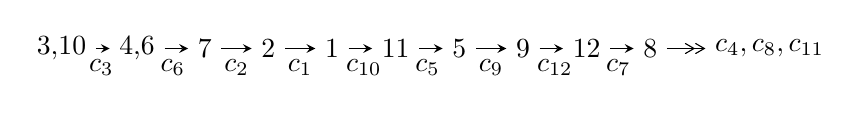
\begin{tikzpicture}[x=23pt, y=7pt]
	% node
	\node (A0) at (-1/8, 0) {3,10};
	\node (A1) at (17/16, 0) {4,6};
	\node (A2) at (17/8, 0) {7};
	\node (A3) at (25/8, 0) {2};
	\node (A4) at (33/8, 0) {1};
	\node (A5) at (41/8, 0) {11};
	\node (A6) at (49/8, 0) {5};
	\node (A7) at (57/8, 0) {9};
	\node (A8) at (65/8, 0) {12};
	\node (A9) at (73/8, 0) {8};
	\node (C1) at (1/2, -1) {$c_{3}$};
	\node (C2) at (13/8, -1) {$c_{6}$};
	\node (C3) at (21/8, -1) {$c_{2}$};
	\node (C4) at (29/8, -1) {$c_{1}$};
	\node (C5) at (37/8, -1) {$c_{10}$};
	\node (C6) at (45/8, -1) {$c_{5}$};
	\node (C7) at (53/8, -1) {$c_{9}$};
	\node (C8) at (61/8, -1) {$c_{12}$};
	\node (C9) at (69/8, -1) {$c_{7}$};
	\node (A10) at (11, 0) {$c_{4},c_{8},c_{11}$};

	% edge
	\draw[->,>=stealth]	
	(A0) edge (A1) (A1) edge (A2) (A2) edge (A3) (A3) edge (A4) (A4) edge (A5) (A5) edge (A6) (A6) edge (A7) (A7) edge (A8) (A8) edge (A9) ;
	\draw[->>,>={angle 60}]	
	(A9) edge (A10);
\end{tikzpicture} \\ 

\end{tabular} \\

\footnotetext{
The image of knot diagram is generated by the software ``\textbf{Draw programme}" developed by Andrew Bartholomew(\url{http://www.layer8.co.uk/maths/draw/index.htm\#Running-draw}), where we modified some parts for our purpose(\url{https://github.com/CATsTAILs/LinksPainter}).
}\phantom \\ \newline 
\centering \textbf{Ideals for irreducible components\footnotemark of $X_{\text{par}}$} 
 
\begin{align*}
I^u_{1}&=\langle 
-2.22257\times10^{23} u^{34}+1.20633\times10^{24} u^{33}+\cdots+9.94460\times10^{24} b+2.05358\times10^{25},\\
\phantom{I^u_{1}}&\phantom{= \langle  }5.94554\times10^{24} u^{34}-9.98345\times10^{24} u^{33}+\cdots+3.97784\times10^{25} a-1.87822\times10^{26},\;u^{35}- u^{34}+\cdots+16 u+8\rangle \\
I^u_{2}&=\langle 
b+1,\;4 a^3+2 a^2 u-4 a- u,\;u^2+2\rangle \\
\\
I^v_{1}&=\langle 
a,\;b-1,\;v^3- v^2+2 v-1\rangle \\
\end{align*}
\raggedright * 3 irreducible components of $\dim_{\mathbb{C}}=0$, with total 44 representations.\\
\footnotetext{All coefficients of polynomials are rational numbers. But the coefficients are sometimes approximated in decimal forms when there is not enough margin.}
\newpage
\renewcommand{\arraystretch}{1}
\centering \section*{I. $I^u_{1}= \langle -2.22\times10^{23} u^{34}+1.21\times10^{24} u^{33}+\cdots+9.94\times10^{24} b+2.05\times10^{25},\;5.95\times10^{24} u^{34}-9.98\times10^{24} u^{33}+\cdots+3.98\times10^{25} a-1.88\times10^{26},\;u^{35}- u^{34}+\cdots+16 u+8 \rangle$}
\flushleft \textbf{(i) Arc colorings}\\
\begin{tabular}{m{7pt} m{180pt} m{7pt} m{180pt} }
\flushright $a_{3}=$&$\begin{pmatrix}1\\0\end{pmatrix}$ \\
\flushright $a_{10}=$&$\begin{pmatrix}0\\u\end{pmatrix}$ \\
\flushright $a_{4}=$&$\begin{pmatrix}1\\u^2\end{pmatrix}$ \\
\flushright $a_{6}=$&$\begin{pmatrix}-0.149467 u^{34}+0.250977 u^{33}+\cdots+0.744011 u+4.72171\\0.0223495 u^{34}-0.121305 u^{33}+\cdots-3.13828 u-2.06502\end{pmatrix}$ \\
\flushright $a_{7}=$&$\begin{pmatrix}-0.149467 u^{34}+0.250977 u^{33}+\cdots+0.744011 u+4.72171\\-0.0135884 u^{34}-0.0414490 u^{33}+\cdots-2.70986 u-1.25294\end{pmatrix}$ \\
\flushright $a_{2}=$&$\begin{pmatrix}-0.135878 u^{34}+0.292426 u^{33}+\cdots+3.45387 u+5.97465\\0.0244551 u^{34}-0.00480744 u^{33}+\cdots+1.29212 u+0.000559791\end{pmatrix}$ \\
\flushright $a_{1}=$&$\begin{pmatrix}-0.111423 u^{34}+0.287618 u^{33}+\cdots+4.74599 u+5.97521\\0.0244551 u^{34}-0.00480744 u^{33}+\cdots+1.29212 u+0.000559791\end{pmatrix}$ \\
\flushright $a_{11}=$&$\begin{pmatrix}0.182308 u^{34}-0.0553187 u^{33}+\cdots+19.9927 u+4.90487\\-0.169723 u^{34}+0.180211 u^{33}+\cdots-4.99372 u-0.555765\end{pmatrix}$ \\
\flushright $a_{5}=$&$\begin{pmatrix}u^2+1\\u^4+2 u^2\end{pmatrix}$ \\
\flushright $a_{9}=$&$\begin{pmatrix}u\\u^3+u\end{pmatrix}$ \\
\flushright $a_{12}=$&$\begin{pmatrix}0.146821 u^{34}-0.205755 u^{33}+\cdots+3.25395 u-3.12378\\-0.115099 u^{34}+0.0771834 u^{33}+\cdots-4.79628 u-1.53754\end{pmatrix}$ \\
\flushright $a_{8}=$&$\begin{pmatrix}- u^3-2 u\\- u^3- u\end{pmatrix}$\\&\end{tabular}
\flushleft \textbf{(ii) Obstruction class $= -1$}\\~\\
\flushleft \textbf{(iii) Cusp Shapes $= -\frac{14744603574080800564971959}{19889209336976177776682620} u^{34}+\frac{19140376741824556567023511}{19889209336976177776682620} u^{33}+\cdots-\frac{13143547959375290290172530}{994460466848808888834131} u+\frac{1519825404502265762057644}{4972302334244044444170655}$}\\~\\
\newpage\renewcommand{\arraystretch}{1}
\flushleft \textbf{(iv) u-Polynomials at the component}\newline \\
\begin{tabular}{m{50pt}|m{274pt}}
Crossings & \hspace{64pt}u-Polynomials at each crossing \\
\hline $$\begin{aligned}c_{1}\end{aligned}$$&$\begin{aligned}
&u^{35}+8 u^{34}+\cdots-52 u+1
\end{aligned}$\\
\hline $$\begin{aligned}c_{2},c_{5}\end{aligned}$$&$\begin{aligned}
&u^{35}+4 u^{34}+\cdots-4 u+1
\end{aligned}$\\
\hline $$\begin{aligned}c_{3},c_{4},c_{9}\end{aligned}$$&$\begin{aligned}
&u^{35}- u^{34}+\cdots+16 u+8
\end{aligned}$\\
\hline $$\begin{aligned}c_{6}\end{aligned}$$&$\begin{aligned}
&u^{35}-2 u^{34}+\cdots+21 u+3
\end{aligned}$\\
\hline $$\begin{aligned}c_{7},c_{11}\end{aligned}$$&$\begin{aligned}
&u^{35}+2 u^{34}+\cdots+9 u+3
\end{aligned}$\\
\hline $$\begin{aligned}c_{8}\end{aligned}$$&$\begin{aligned}
&u^{35}+u^{34}+\cdots+480 u+200
\end{aligned}$\\
\hline $$\begin{aligned}c_{10},c_{12}\end{aligned}$$&$\begin{aligned}
&u^{35}-14 u^{34}+\cdots+129 u-9
\end{aligned}$\\
\hline
\end{tabular}\\~\\
\newpage\renewcommand{\arraystretch}{1}
\flushleft \textbf{(v) Riley Polynomials at the component}\newline \\
\begin{tabular}{m{50pt}|m{274pt}}
Crossings & \hspace{64pt}Riley Polynomials at each crossing \\
\hline $$\begin{aligned}c_{1}\end{aligned}$$&$\begin{aligned}
&y^{35}+48 y^{34}+\cdots+1020 y-1
\end{aligned}$\\
\hline $$\begin{aligned}c_{2},c_{5}\end{aligned}$$&$\begin{aligned}
&y^{35}-8 y^{34}+\cdots-52 y-1
\end{aligned}$\\
\hline $$\begin{aligned}c_{3},c_{4},c_{9}\end{aligned}$$&$\begin{aligned}
&y^{35}+49 y^{34}+\cdots-768 y-64
\end{aligned}$\\
\hline $$\begin{aligned}c_{6}\end{aligned}$$&$\begin{aligned}
&y^{35}-54 y^{34}+\cdots-15 y-9
\end{aligned}$\\
\hline $$\begin{aligned}c_{7},c_{11}\end{aligned}$$&$\begin{aligned}
&y^{35}-14 y^{34}+\cdots+129 y-9
\end{aligned}$\\
\hline $$\begin{aligned}c_{8}\end{aligned}$$&$\begin{aligned}
&y^{35}+133 y^{34}+\cdots-12598400 y-40000
\end{aligned}$\\
\hline $$\begin{aligned}c_{10},c_{12}\end{aligned}$$&$\begin{aligned}
&y^{35}+18 y^{34}+\cdots+2313 y-81
\end{aligned}$\\
\hline
\end{tabular}\\~\\
\newpage\flushleft \textbf{(vi) Complex Volumes and Cusp Shapes}
$$\begin{array}{c|c|c}  
\text{Solutions to }I^u_{1}& \I (\text{vol} + \sqrt{-1}CS) & \text{Cusp shape}\\
 \hline 
\begin{aligned}
u &= \phantom{-}0.001709 + 0.955912 I \\
a &= \phantom{-}0.185156 - 0.791460 I \\
b &= -0.661252 + 0.559258 I\end{aligned}
 & \phantom{-}1.60959 + 1.37990 I & -0.61653 - 3.70044 I \\ \hline\begin{aligned}
u &= \phantom{-}0.001709 - 0.955912 I \\
a &= \phantom{-}0.185156 + 0.791460 I \\
b &= -0.661252 - 0.559258 I\end{aligned}
 & \phantom{-}1.60959 - 1.37990 I & -0.61653 + 3.70044 I \\ \hline\begin{aligned}
u &= -0.457643 + 0.944024 I \\
a &= -0.498093 - 1.222730 I \\
b &= -0.873919 + 0.740811 I\end{aligned}
 & \phantom{-}1.28798 + 3.57056 I & -1.83989 - 3.72840 I \\ \hline\begin{aligned}
u &= -0.457643 - 0.944024 I \\
a &= -0.498093 + 1.222730 I \\
b &= -0.873919 - 0.740811 I\end{aligned}
 & \phantom{-}1.28798 - 3.57056 I & -1.83989 + 3.72840 I \\ \hline\begin{aligned}
u &= \phantom{-}0.578123 + 1.001790 I \\
a &= -0.641074 + 1.123880 I \\
b &= -0.937353 - 0.867983 I\end{aligned}
 & \phantom{-}2.89503 - 8.89111 I & \phantom{-}0.41854 + 7.86310 I \\ \hline\begin{aligned}
u &= \phantom{-}0.578123 - 1.001790 I \\
a &= -0.641074 - 1.123880 I \\
b &= -0.937353 + 0.867983 I\end{aligned}
 & \phantom{-}2.89503 + 8.89111 I & \phantom{-}0.41854 - 7.86310 I \\ \hline\begin{aligned}
u &= -0.280567 + 1.198240 I \\
a &= \phantom{-}0.212983 + 0.307706 I \\
b &= -0.848880 - 0.653452 I\end{aligned}
 & \phantom{-}2.89532 + 2.93605 I & \phantom{-}1.67114 - 3.26620 I \\ \hline\begin{aligned}
u &= -0.280567 - 1.198240 I \\
a &= \phantom{-}0.212983 - 0.307706 I \\
b &= -0.848880 + 0.653452 I\end{aligned}
 & \phantom{-}2.89532 - 2.93605 I & \phantom{-}1.67114 + 3.26620 I \\ \hline\begin{aligned}
u &= \phantom{-}0.746902 + 0.064874 I \\
a &= \phantom{-}0.763197 + 0.046917 I \\
b &= \phantom{-}0.618050 + 0.742602 I\end{aligned}
 & -0.31975 - 4.37952 I & -1.83091 + 6.07452 I \\ \hline\begin{aligned}
u &= \phantom{-}0.746902 - 0.064874 I \\
a &= \phantom{-}0.763197 - 0.046917 I \\
b &= \phantom{-}0.618050 - 0.742602 I\end{aligned}
 & -0.31975 + 4.37952 I & -1.83091 - 6.07452 I\\
 \hline 
 \end{array}$$\newpage$$\begin{array}{c|c|c}  
\text{Solutions to }I^u_{1}& \I (\text{vol} + \sqrt{-1}CS) & \text{Cusp shape}\\
 \hline 
\begin{aligned}
u &= \phantom{-}0.353706 + 1.218390 I \\
a &= -0.474249 + 0.899612 I \\
b &= -0.572481 - 0.845888 I\end{aligned}
 & \phantom{-}6.57185 - 2.11496 I & \phantom{-}5.70868 + 2.44246 I \\ \hline\begin{aligned}
u &= \phantom{-}0.353706 - 1.218390 I \\
a &= -0.474249 - 0.899612 I \\
b &= -0.572481 + 0.845888 I\end{aligned}
 & \phantom{-}6.57185 + 2.11496 I & \phantom{-}5.70868 - 2.44246 I \\ \hline\begin{aligned}
u &= \phantom{-}0.398585 + 0.473638 I \\
a &= \phantom{-}0.800117 - 0.238876 I \\
b &= -0.139739 + 0.561536 I\end{aligned}
 & \phantom{-}1.46027 + 0.77126 I & \phantom{-}3.61366 - 0.98435 I \\ \hline\begin{aligned}
u &= \phantom{-}0.398585 - 0.473638 I \\
a &= \phantom{-}0.800117 + 0.238876 I \\
b &= -0.139739 - 0.561536 I\end{aligned}
 & \phantom{-}1.46027 - 0.77126 I & \phantom{-}3.61366 + 0.98435 I \\ \hline\begin{aligned}
u &= -0.090108 + 0.598555 I \\
a &= \phantom{-}1.184960 + 0.064358 I \\
b &= \phantom{-}1.219850 + 0.040491 I\end{aligned}
 & -3.56638 - 2.55876 I & -1.13575 + 2.02591 I \\ \hline\begin{aligned}
u &= -0.090108 - 0.598555 I \\
a &= \phantom{-}1.184960 - 0.064358 I \\
b &= \phantom{-}1.219850 - 0.040491 I\end{aligned}
 & -3.56638 + 2.55876 I & -1.13575 - 2.02591 I \\ \hline\begin{aligned}
u &= \phantom{-}0.031695 + 1.407050 I \\
a &= -0.911900 + 0.239123 I \\
b &= -0.046000 - 0.170713 I\end{aligned}
 & \phantom{-}1.93564 + 2.80926 I & \phantom{-0.000000 } 0 \\ \hline\begin{aligned}
u &= \phantom{-}0.031695 - 1.407050 I \\
a &= -0.911900 - 0.239123 I \\
b &= -0.046000 + 0.170713 I\end{aligned}
 & \phantom{-}1.93564 - 2.80926 I & \phantom{-0.000000 } 0 \\ \hline\begin{aligned}
u &= -0.576386 + 0.100273 I \\
a &= \phantom{-}0.859064 + 0.075571 I \\
b &= \phantom{-}0.794836 + 0.430575 I\end{aligned}
 & -1.361170 + 0.009026 I & -6.02384 - 1.12650 I \\ \hline\begin{aligned}
u &= -0.576386 - 0.100273 I \\
a &= \phantom{-}0.859064 - 0.075571 I \\
b &= \phantom{-}0.794836 - 0.430575 I\end{aligned}
 & -1.361170 - 0.009026 I & -6.02384 + 1.12650 I\\
 \hline 
 \end{array}$$\newpage$$\begin{array}{c|c|c}  
\text{Solutions to }I^u_{1}& \I (\text{vol} + \sqrt{-1}CS) & \text{Cusp shape}\\
 \hline 
\begin{aligned}
u &= -0.07940 + 1.54042 I \\
a &= \phantom{-}0.1203980 + 0.0430251 I \\
b &= -1.303940 - 0.164109 I\end{aligned}
 & \phantom{-}3.74701 - 1.80891 I & \phantom{-0.000000 } 0 \\ \hline\begin{aligned}
u &= -0.07940 - 1.54042 I \\
a &= \phantom{-}0.1203980 - 0.0430251 I \\
b &= -1.303940 + 0.164109 I\end{aligned}
 & \phantom{-}3.74701 + 1.80891 I & \phantom{-0.000000 } 0 \\ \hline\begin{aligned}
u &= -0.020066 + 0.420369 I \\
a &= \phantom{-}3.70274 - 0.63177 I \\
b &= -0.763223 + 0.037247 I\end{aligned}
 & -4.12675 + 2.92147 I & \phantom{-}3.70844 - 4.07635 I \\ \hline\begin{aligned}
u &= -0.020066 - 0.420369 I \\
a &= \phantom{-}3.70274 + 0.63177 I \\
b &= -0.763223 - 0.037247 I\end{aligned}
 & -4.12675 - 2.92147 I & \phantom{-}3.70844 + 4.07635 I \\ \hline\begin{aligned}
u &= -0.361397\phantom{ +0.000000I} \\
a &= \phantom{-}0.932708\phantom{ +0.000000I} \\
b &= \phantom{-}0.810295\phantom{ +0.000000I}\end{aligned}
 & -1.03588\phantom{ +0.000000I} & -12.2760\phantom{ +0.000000I} \\ \hline\begin{aligned}
u &= -0.14043 + 1.72815 I \\
a &= -0.16477 + 1.41522 I \\
b &= \phantom{-}1.14266 - 0.93268 I\end{aligned}
 & \phantom{-}10.72680 + 6.05251 I & \phantom{-0.000000 } 0 \\ \hline\begin{aligned}
u &= -0.14043 - 1.72815 I \\
a &= -0.16477 - 1.41522 I \\
b &= \phantom{-}1.14266 + 0.93268 I\end{aligned}
 & \phantom{-}10.72680 - 6.05251 I & \phantom{-0.000000 } 0 \\ \hline\begin{aligned}
u &= \phantom{-}0.18174 + 1.73920 I \\
a &= -0.077993 - 1.391040 I \\
b &= \phantom{-}1.23438 + 0.93163 I\end{aligned}
 & \phantom{-}12.4359 - 12.0719 I & \phantom{-0.000000 } 0 \\ \hline\begin{aligned}
u &= \phantom{-}0.18174 - 1.73920 I \\
a &= -0.077993 + 1.391040 I \\
b &= \phantom{-}1.23438 - 0.93163 I\end{aligned}
 & \phantom{-}12.4359 + 12.0719 I & \phantom{-0.000000 } 0 \\ \hline\begin{aligned}
u &= -0.00142 + 1.75473 I \\
a &= -0.393349 + 1.254280 I \\
b &= \phantom{-}0.860192 - 1.095830 I\end{aligned}
 & \phantom{-}11.66250 + 1.36680 I & \phantom{-0.000000 } 0\\
 \hline 
 \end{array}$$\newpage$$\begin{array}{c|c|c}  
\text{Solutions to }I^u_{1}& \I (\text{vol} + \sqrt{-1}CS) & \text{Cusp shape}\\
 \hline 
\begin{aligned}
u &= -0.00142 - 1.75473 I \\
a &= -0.393349 - 1.254280 I \\
b &= \phantom{-}0.860192 + 1.095830 I\end{aligned}
 & \phantom{-}11.66250 - 1.36680 I & \phantom{-0.000000 } 0 \\ \hline\begin{aligned}
u &= -0.05090 + 1.79450 I \\
a &= -0.401616 - 1.156030 I \\
b &= \phantom{-}0.78741 + 1.23198 I\end{aligned}
 & \phantom{-}13.9358 + 4.2732 I & \phantom{-0.000000 } 0 \\ \hline\begin{aligned}
u &= -0.05090 - 1.79450 I \\
a &= -0.401616 + 1.156030 I \\
b &= \phantom{-}0.78741 - 1.23198 I\end{aligned}
 & \phantom{-}13.9358 - 4.2732 I & \phantom{-0.000000 } 0 \\ \hline\begin{aligned}
u &= \phantom{-}0.08516 + 1.80955 I \\
a &= -0.231921 - 1.248780 I \\
b &= \phantom{-}1.08426 + 1.14113 I\end{aligned}
 & \phantom{-}17.6851 - 4.1242 I & \phantom{-0.000000 } 0 \\ \hline\begin{aligned}
u &= \phantom{-}0.08516 - 1.80955 I \\
a &= -0.231921 + 1.248780 I \\
b &= \phantom{-}1.08426 - 1.14113 I\end{aligned}
 & \phantom{-}17.6851 + 4.1242 I & \phantom{-0.000000 } 0\\
 \hline 
 \end{array}$$\newpage\newpage\renewcommand{\arraystretch}{1}
\centering \section*{II. $I^u_{2}= \langle b+1,\;4 a^3+2 a^2 u-4 a- u,\;u^2+2 \rangle$}
\flushleft \textbf{(i) Arc colorings}\\
\begin{tabular}{m{7pt} m{180pt} m{7pt} m{180pt} }
\flushright $a_{3}=$&$\begin{pmatrix}1\\0\end{pmatrix}$ \\
\flushright $a_{10}=$&$\begin{pmatrix}0\\u\end{pmatrix}$ \\
\flushright $a_{4}=$&$\begin{pmatrix}1\\-2\end{pmatrix}$ \\
\flushright $a_{6}=$&$\begin{pmatrix}a\\-1\end{pmatrix}$ \\
\flushright $a_{7}=$&$\begin{pmatrix}a\\2 a-1\end{pmatrix}$ \\
\flushright $a_{2}=$&$\begin{pmatrix}a+1\\-1\end{pmatrix}$ \\
\flushright $a_{1}=$&$\begin{pmatrix}a\\-1\end{pmatrix}$ \\
\flushright $a_{11}=$&$\begin{pmatrix}a^2 u\\- a u+u\end{pmatrix}$ \\
\flushright $a_{5}=$&$\begin{pmatrix}-1\\0\end{pmatrix}$ \\
\flushright $a_{9}=$&$\begin{pmatrix}u\\- u\end{pmatrix}$ \\
\flushright $a_{12}=$&$\begin{pmatrix}a^2 u- a-\frac{1}{2} u\\2 a^2-2 a-1\end{pmatrix}$ \\
\flushright $a_{8}=$&$\begin{pmatrix}0\\- u\end{pmatrix}$\\&\end{tabular}
\flushleft \textbf{(ii) Obstruction class $= 1$}\\~\\
\flushleft \textbf{(iii) Cusp Shapes $= -8 a^2-4 a u+4$}\\~\\
\newpage\renewcommand{\arraystretch}{1}
\flushleft \textbf{(iv) u-Polynomials at the component}\newline \\
\begin{tabular}{m{50pt}|m{274pt}}
Crossings & \hspace{64pt}u-Polynomials at each crossing \\
\hline $$\begin{aligned}c_{1},c_{5}\end{aligned}$$&$\begin{aligned}
&(u-1)^6
\end{aligned}$\\
\hline $$\begin{aligned}c_{2}\end{aligned}$$&$\begin{aligned}
&(u+1)^6
\end{aligned}$\\
\hline $$\begin{aligned}c_{3},c_{4},c_{8}\\c_{9}\end{aligned}$$&$\begin{aligned}
&(u^2+2)^3
\end{aligned}$\\
\hline $$\begin{aligned}c_{6},c_{12}\end{aligned}$$&$\begin{aligned}
&(u^3- u^2+2 u-1)^2
\end{aligned}$\\
\hline $$\begin{aligned}c_{7}\end{aligned}$$&$\begin{aligned}
&(u^3+u^2-1)^2
\end{aligned}$\\
\hline $$\begin{aligned}c_{10}\end{aligned}$$&$\begin{aligned}
&(u^3+u^2+2 u+1)^2
\end{aligned}$\\
\hline $$\begin{aligned}c_{11}\end{aligned}$$&$\begin{aligned}
&(u^3- u^2+1)^2
\end{aligned}$\\
\hline
\end{tabular}\\~\\
\newpage\renewcommand{\arraystretch}{1}
\flushleft \textbf{(v) Riley Polynomials at the component}\newline \\
\begin{tabular}{m{50pt}|m{274pt}}
Crossings & \hspace{64pt}Riley Polynomials at each crossing \\
\hline $$\begin{aligned}c_{1},c_{2},c_{5}\end{aligned}$$&$\begin{aligned}
&(y-1)^6
\end{aligned}$\\
\hline $$\begin{aligned}c_{3},c_{4},c_{8}\\c_{9}\end{aligned}$$&$\begin{aligned}
&(y+2)^6
\end{aligned}$\\
\hline $$\begin{aligned}c_{6},c_{10},c_{12}\end{aligned}$$&$\begin{aligned}
&(y^3+3 y^2+2 y-1)^2
\end{aligned}$\\
\hline $$\begin{aligned}c_{7},c_{11}\end{aligned}$$&$\begin{aligned}
&(y^3- y^2+2 y-1)^2
\end{aligned}$\\
\hline
\end{tabular}\\~\\
\newpage\flushleft \textbf{(vi) Complex Volumes and Cusp Shapes}
$$\begin{array}{c|c|c}  
\text{Solutions to }I^u_{2}& \I (\text{vol} + \sqrt{-1}CS) & \text{Cusp shape}\\
 \hline 
\begin{aligned}
u &= \phantom{-0.000000 -}1.414210 I \\
a &= \phantom{-}0.924288 - 0.152084 I \\
b &= -1.00000\phantom{ +0.000000I}\end{aligned}
 & \phantom{-}0.26574 + 2.82812 I & -3.50976 - 2.97945 I \\ \hline\begin{aligned}
u &= \phantom{-0.000000 -}1.414210 I \\
a &= -0.924288 - 0.152084 I \\
b &= -1.00000\phantom{ +0.000000I}\end{aligned}
 & \phantom{-}0.26574 - 2.82812 I & -3.50976 + 2.97945 I \\ \hline\begin{aligned}
u &= \phantom{-0.000000 -}1.414210 I \\
a &= \phantom{-0.000000 } -0.402938 I \\
b &= -1.00000\phantom{ +0.000000I}\end{aligned}
 & \phantom{-}4.40332\phantom{ +0.000000I} & \phantom{-}3.01950\phantom{ +0.000000I} \\ \hline\begin{aligned}
u &= \phantom{-0.000000 } -1.414210 I \\
a &= \phantom{-}0.924288 + 0.152084 I \\
b &= -1.00000\phantom{ +0.000000I}\end{aligned}
 & \phantom{-}0.26574 - 2.82812 I & -3.50976 + 2.97945 I \\ \hline\begin{aligned}
u &= \phantom{-0.000000 } -1.414210 I \\
a &= -0.924288 + 0.152084 I \\
b &= -1.00000\phantom{ +0.000000I}\end{aligned}
 & \phantom{-}0.26574 + 2.82812 I & -3.50976 - 2.97945 I \\ \hline\begin{aligned}
u &= \phantom{-0.000000 } -1.414210 I \\
a &= \phantom{-0.000000 -}0.402938 I \\
b &= -1.00000\phantom{ +0.000000I}\end{aligned}
 & \phantom{-}4.40332\phantom{ +0.000000I} & \phantom{-}3.01950\phantom{ +0.000000I}\\
 \hline 
 \end{array}$$\newpage\newpage\renewcommand{\arraystretch}{1}
\centering \section*{III. $I^v_{1}= \langle a,\;b-1,\;v^3- v^2+2 v-1 \rangle$}
\flushleft \textbf{(i) Arc colorings}\\
\begin{tabular}{m{7pt} m{180pt} m{7pt} m{180pt} }
\flushright $a_{3}=$&$\begin{pmatrix}1\\0\end{pmatrix}$ \\
\flushright $a_{10}=$&$\begin{pmatrix}v\\0\end{pmatrix}$ \\
\flushright $a_{4}=$&$\begin{pmatrix}1\\0\end{pmatrix}$ \\
\flushright $a_{6}=$&$\begin{pmatrix}0\\1\end{pmatrix}$ \\
\flushright $a_{7}=$&$\begin{pmatrix}v^2\\1\end{pmatrix}$ \\
\flushright $a_{2}=$&$\begin{pmatrix}1\\-1\end{pmatrix}$ \\
\flushright $a_{1}=$&$\begin{pmatrix}0\\-1\end{pmatrix}$ \\
\flushright $a_{11}=$&$\begin{pmatrix}v\\- v\end{pmatrix}$ \\
\flushright $a_{5}=$&$\begin{pmatrix}1\\0\end{pmatrix}$ \\
\flushright $a_{9}=$&$\begin{pmatrix}v\\0\end{pmatrix}$ \\
\flushright $a_{12}=$&$\begin{pmatrix}v^2\\- v^2-1\end{pmatrix}$ \\
\flushright $a_{8}=$&$\begin{pmatrix}v\\0\end{pmatrix}$\\&\end{tabular}
\flushleft \textbf{(ii) Obstruction class $= 1$}\\~\\
\flushleft \textbf{(iii) Cusp Shapes $= 10 v^2-6 v+6$}\\~\\
\newpage\renewcommand{\arraystretch}{1}
\flushleft \textbf{(iv) u-Polynomials at the component}\newline \\
\begin{tabular}{m{50pt}|m{274pt}}
Crossings & \hspace{64pt}u-Polynomials at each crossing \\
\hline $$\begin{aligned}c_{1},c_{2}\end{aligned}$$&$\begin{aligned}
&(u-1)^3
\end{aligned}$\\
\hline $$\begin{aligned}c_{3},c_{4},c_{8}\\c_{9}\end{aligned}$$&$\begin{aligned}
&u^3
\end{aligned}$\\
\hline $$\begin{aligned}c_{5}\end{aligned}$$&$\begin{aligned}
&(u+1)^3
\end{aligned}$\\
\hline $$\begin{aligned}c_{6},c_{10}\end{aligned}$$&$\begin{aligned}
&u^3+u^2+2 u+1
\end{aligned}$\\
\hline $$\begin{aligned}c_{7}\end{aligned}$$&$\begin{aligned}
&u^3- u^2+1
\end{aligned}$\\
\hline $$\begin{aligned}c_{11}\end{aligned}$$&$\begin{aligned}
&u^3+u^2-1
\end{aligned}$\\
\hline $$\begin{aligned}c_{12}\end{aligned}$$&$\begin{aligned}
&u^3- u^2+2 u-1
\end{aligned}$\\
\hline
\end{tabular}\\~\\
\newpage\renewcommand{\arraystretch}{1}
\flushleft \textbf{(v) Riley Polynomials at the component}\newline \\
\begin{tabular}{m{50pt}|m{274pt}}
Crossings & \hspace{64pt}Riley Polynomials at each crossing \\
\hline $$\begin{aligned}c_{1},c_{2},c_{5}\end{aligned}$$&$\begin{aligned}
&(y-1)^3
\end{aligned}$\\
\hline $$\begin{aligned}c_{3},c_{4},c_{8}\\c_{9}\end{aligned}$$&$\begin{aligned}
&y^3
\end{aligned}$\\
\hline $$\begin{aligned}c_{6},c_{10},c_{12}\end{aligned}$$&$\begin{aligned}
&y^3+3 y^2+2 y-1
\end{aligned}$\\
\hline $$\begin{aligned}c_{7},c_{11}\end{aligned}$$&$\begin{aligned}
&y^3- y^2+2 y-1
\end{aligned}$\\
\hline
\end{tabular}\\~\\
\newpage\flushleft \textbf{(vi) Complex Volumes and Cusp Shapes}
$$\begin{array}{c|c|c}  
\text{Solutions to }I^v_{1}& \I (\text{vol} + \sqrt{-1}CS) & \text{Cusp shape}\\
 \hline 
\begin{aligned}
v &= \phantom{-}0.215080 + 1.307140 I \\
a &= \phantom{-0.000000 } 0 \\
b &= \phantom{-}1.00000\phantom{ +0.000000I}\end{aligned}
 & -4.66906 + 2.82812 I & -11.91407 - 2.22005 I \\ \hline\begin{aligned}
v &= \phantom{-}0.215080 - 1.307140 I \\
a &= \phantom{-0.000000 } 0 \\
b &= \phantom{-}1.00000\phantom{ +0.000000I}\end{aligned}
 & -4.66906 - 2.82812 I & -11.91407 + 2.22005 I \\ \hline\begin{aligned}
v &= \phantom{-}0.569840\phantom{ +0.000000I} \\
a &= \phantom{-0.000000 } 0 \\
b &= \phantom{-}1.00000\phantom{ +0.000000I}\end{aligned}
 & -0.531480\phantom{ +0.000000I} & \phantom{-}5.82810\phantom{ +0.000000I}\\
 \hline 
 \end{array}$$\newpage
\newpage\renewcommand{\arraystretch}{1}
\centering \section*{ IV. u-Polynomials}
\begin{tabular}{m{50pt}|m{274pt}}
Crossings & \hspace{64pt}u-Polynomials at each crossing \\
\hline $$\begin{aligned}c_{1}\end{aligned}$$&$\begin{aligned}
&((u-1)^9)(u^{35}+8 u^{34}+\cdots-52 u+1)
\end{aligned}$\\
\hline $$\begin{aligned}c_{2}\end{aligned}$$&$\begin{aligned}
&((u-1)^3)(u+1)^6(u^{35}+4 u^{34}+\cdots-4 u+1)
\end{aligned}$\\
\hline $$\begin{aligned}c_{3},c_{4},c_{9}\end{aligned}$$&$\begin{aligned}
&u^3(u^2+2)^3(u^{35}- u^{34}+\cdots+16 u+8)
\end{aligned}$\\
\hline $$\begin{aligned}c_{5}\end{aligned}$$&$\begin{aligned}
&((u-1)^6)(u+1)^3(u^{35}+4 u^{34}+\cdots-4 u+1)
\end{aligned}$\\
\hline $$\begin{aligned}c_{6}\end{aligned}$$&$\begin{aligned}
&((u^3- u^2+2 u-1)^2)(u^3+u^2+2 u+1)(u^{35}-2 u^{34}+\cdots+21 u+3)
\end{aligned}$\\
\hline $$\begin{aligned}c_{7}\end{aligned}$$&$\begin{aligned}
&(u^3- u^2+1)(u^3+u^2-1)^2(u^{35}+2 u^{34}+\cdots+9 u+3)
\end{aligned}$\\
\hline $$\begin{aligned}c_{8}\end{aligned}$$&$\begin{aligned}
&u^3(u^2+2)^3(u^{35}+u^{34}+\cdots+480 u+200)
\end{aligned}$\\
\hline $$\begin{aligned}c_{10}\end{aligned}$$&$\begin{aligned}
&((u^3+u^2+2 u+1)^3)(u^{35}-14 u^{34}+\cdots+129 u-9)
\end{aligned}$\\
\hline $$\begin{aligned}c_{11}\end{aligned}$$&$\begin{aligned}
&((u^3- u^2+1)^2)(u^3+u^2-1)(u^{35}+2 u^{34}+\cdots+9 u+3)
\end{aligned}$\\
\hline $$\begin{aligned}c_{12}\end{aligned}$$&$\begin{aligned}
&((u^3- u^2+2 u-1)^3)(u^{35}-14 u^{34}+\cdots+129 u-9)
\end{aligned}$\\
\hline
\end{tabular}\newpage\renewcommand{\arraystretch}{1}
\centering \section*{ V. Riley Polynomials}
\begin{tabular}{m{50pt}|m{274pt}}
Crossings & \hspace{64pt}Riley Polynomials at each crossing \\
\hline $$\begin{aligned}c_{1}\end{aligned}$$&$\begin{aligned}
&((y-1)^9)(y^{35}+48 y^{34}+\cdots+1020 y-1)
\end{aligned}$\\
\hline $$\begin{aligned}c_{2},c_{5}\end{aligned}$$&$\begin{aligned}
&((y-1)^9)(y^{35}-8 y^{34}+\cdots-52 y-1)
\end{aligned}$\\
\hline $$\begin{aligned}c_{3},c_{4},c_{9}\end{aligned}$$&$\begin{aligned}
&y^3(y+2)^6(y^{35}+49 y^{34}+\cdots-768 y-64)
\end{aligned}$\\
\hline $$\begin{aligned}c_{6}\end{aligned}$$&$\begin{aligned}
&((y^3+3 y^2+2 y-1)^3)(y^{35}-54 y^{34}+\cdots-15 y-9)
\end{aligned}$\\
\hline $$\begin{aligned}c_{7},c_{11}\end{aligned}$$&$\begin{aligned}
&((y^3- y^2+2 y-1)^3)(y^{35}-14 y^{34}+\cdots+129 y-9)
\end{aligned}$\\
\hline $$\begin{aligned}c_{8}\end{aligned}$$&$\begin{aligned}
&y^3(y+2)^6(y^{35}+133 y^{34}+\cdots-1.25984\times10^{7} y-40000)
\end{aligned}$\\
\hline $$\begin{aligned}c_{10},c_{12}\end{aligned}$$&$\begin{aligned}
&((y^3+3 y^2+2 y-1)^3)(y^{35}+18 y^{34}+\cdots+2313 y-81)
\end{aligned}$\\
\hline
\end{tabular}
\vskip 2pc
\end{document}